\documentclass[11pt]{article}
\usepackage[a4paper,margin=25mm]{geometry}
\usepackage{amsmath,amssymb,amsthm,mathtools}
\usepackage{booktabs,array,float}
\usepackage{xcolor}
\usepackage{tikz}
\usetikzlibrary{arrows.meta,positioning}
\usepackage[most]{tcolorbox}
\usepackage[hyphens]{url}
\usepackage[numbers,sort&compress]{natbib}
\usepackage{hyperref}
\hypersetup{colorlinks=true,linkcolor=blue!50!black,citecolor=blue!50!black,urlcolor=blue!60!black,
  pdftitle={Instanton lifts and the quantum product in pure N=1 Yang-Mills theory},pdfauthor={Botao Li}}
\numberwithin{equation}{section}
\numberwithin{figure}{section}
\numberwithin{table}{section}
\newtheorem{theorem}{Theorem}[section]
\newtheorem{proposition}[theorem]{Proposition}
\newtheorem{lemma}[theorem]{Lemma}
\newtheorem{corollary}[theorem]{Corollary}
\newtheorem{conjecture}[theorem]{Conjecture}
\theoremstyle{definition}
\newtheorem{definition}[theorem]{Definition}
\newtheorem{assumption}[theorem]{Assumption}
\newtheorem{example}[theorem]{Example}
\newtheorem{remark}[theorem]{Remark}
\newtcolorbox{proofbox}{breakable,enhanced,colback=white,colframe=black!28,boxrule=0.4pt,arc=1pt,
  left=5pt,right=5pt,top=3pt,bottom=3pt,before skip=6pt,after skip=8pt,parbox=false}
\newcommand{\Qp}{\mathbf Q}
\newcommand{\Qi}{Q_{1\text{-}\mathrm{inst}}}
\newcommand{\Ep}{E_\infty^{\mathrm{pert}}}
\allowdisplaybreaks[3]
\setlength{\parskip}{3pt}
\setlength{\emergencystretch}{2em}
\renewcommand{\arraystretch}{1.25}
\title{Instanton lifts and the quantum product\\ in pure $\mathcal N=1$ Yang--Mills theory}
\author{Botao Li\\[4pt]{\normalsize Peking University}}
\date{}
\begin{document}
\maketitle
\begin{abstract}
The local operators of pure $\mathcal N=1$ Yang--Mills theory that are annihilated by one supercharge form, in perturbation theory, an infinite-dimensional cohomology, while the infrared theory has $N$ gapped vacua and no local operators beyond the powers of the gaugino bilinear. Budzik, Gaiotto, Kulp, Williams, Wu and Yu conjectured that instantons remove the difference, pairing the perturbative classes through a one-instanton correction of the supercharge. We show that this correction is determined, on the classes annihilated by the gaugino bilinear, by a single number: the constant $\nu$ in the relation between the $N$-th power of the gaugino bilinear and the strong-coupling scale. The relation makes multiplication by the gaugino bilinear invertible up to homotopy; the homotopy defines a triple product of Massey type, and the one-instanton correction is $-\nu$ times its inverse. A class annihilated by the gaugino bilinear therefore has a partner, which we construct with the loop-corrected supercharge and the quantum product of the holomorphic twist. We compute the partners explicitly: for $SU(2)$, of the first three classes formed by the gaugino bilinear and even powers of the field strength, using the supercharge through three loops and the product through two loops; for $SU(3)$, of the first such class. The partners are the classes found by an extended perturbative census. The same computation gives the products among these classes, which are invisible at the level of leading terms. A one-instanton calculation gives the constant: the gaugino zero modes saturate two insertions of the bilinear at separate points, and their correlator is independent of the separation. Massive adjoint or fundamental matter leaves every perturbative page unchanged in the range computed, and the same relation then reproduces the two Seiberg--Witten vacua and the Affleck--Dine--Seiberg vacuum.
\end{abstract}
{\small\setcounter{tocdepth}{2}\tableofcontents}
\bigskip

\section{Introduction}\label{sec-intro}

In a four-dimensional $\mathcal N=1$ theory, the local operators annihilated by one supercharge $Q$, modulo $Q$-exact operators, are the semi-chiral operators. Their cohomology contains the chiral ring and is invariant along the renormalization group flow, so it can be compared between an ultraviolet Lagrangian description and the infrared phase \cite[Section~1]{semichiral}. For pure $SU(N)$ Yang--Mills theory the two sides look very different. In the ultraviolet, the holomorphic twist presents the cohomology as that of gauge-invariant polynomials in the derivatives of two fields $b$ and $c$, with a differential $\Qp=\sum_n\hbar^nQ_n$ whose loop corrections are finite and computable \cite{semichiral,BK,LLCh}; its cohomology is infinite dimensional. In the infrared, the theory confines and has $N$ gapped vacua, distinguished by the expectation value of the gaugino bilinear $C_0$; the only local operators are the functions on this set of vacua, the span of $1,C_0,\dots,C_0^{N-1}$ with $C_0^N$ proportional to $\Lambda^{3N}$ \cite{VY}.

Budzik, Gaiotto, Kulp, Williams, Wu and Yu proposed that instantons account for the difference \cite[Section~8]{semichiral}. The exact supercharge is $\Qp$ plus a one-instanton term $\Lambda^{3N}\Qi$ plus higher instanton numbers; $\Qi$ lowers the twisted spin by $2N$ and raises the cohomological degree by one, and it should pair up every perturbative class other than the powers of $C_0$. For $SU(2)$ they computed the perturbative cohomology up to fourteen derivatives and observed that the charges of the classes are compatible with such a pairing \cite[Equation~(8.11)]{semichiral}; two classes had their candidate partners above the computed range, and for $SU(3)$ the first candidate partner was out of reach. The operator $\Qi$ itself was left undetermined.

This paper determines $\Qi$ on the classes annihilated by $C_0$ and computes it on the first classes. The starting point is that the exact relation
\begin{equation}\label{eq-intro-relation}
[C_0]^N=\nu\,\Lambda^{3N}
\end{equation}
is an identity between operators acting on the cohomology: with $L$ the multiplication by $C_0$ and $x_N$ a perturbative primitive of $C_0^N$, there is an operator $h$, equal to multiplication by $x_N$ at leading order, such that
\begin{equation}\label{eq-intro-homotopy}
Qh+hQ=L^N-\nu\,\Lambda^{3N}.
\end{equation}
A perturbative class $a$ with $C_0\,a=0$ then defines a second class, the triple product $\langle C_0^{N-1},C_0,a\rangle$, and expanding \eqref{eq-intro-homotopy} to first order in $\Lambda^{3N}$ gives our main result (Theorem~\ref{thm-mechanism}):
\begin{equation}\label{eq-intro-main}
\Qi\,\langle C_0^{N-1},C_0,a\rangle+\langle C_0^{N-1},C_0,\Qi\,a\rangle=-\nu\,a .
\end{equation}
If $a$ is not itself a multiple of $C_0^{N-1}$, its triple product is a nonzero perturbative class, and the instanton maps it to $-\nu\,a$: both are removed from the exact cohomology. The constant $\nu$ is the only non-perturbative input.\footnote{The identity \eqref{eq-intro-homotopy} assumes that the exact supercharge is a derivation of an exact product of local operators that is associative up to homotopy, as the perturbative supercharge is for the quantum product (Assumption~\ref{ass-exact}).}

The operators $L$ and $h$ are multiplications in the sense of the quantum product $\star$ of the twisted theory: the ordinary product of two local operators is compatible with $Q_0$ alone, and the loop corrections of the supercharge require loop corrections of the product. The product, its Leibniz rule and its ring laws on cohomology were established at every loop order in \cite{LLCh}, building on the marked operations of Gaiotto, Kulp and Wu \cite{higher}; its discussion closes by naming the interplay of instanton lifts with the product as an open direction, and the present paper takes it up. We evaluate the product on the fields $b$ and $c$ through two loops (Section~\ref{sec-product}); these terms are needed because a triple product has its leading component removed by an exact term, so that the class sits one or more loop orders below.

With these tools we obtain the following.

\emph{Explicit pairs.} For $SU(2)$ the perturbative classes include a tower $C_2,C_4,C_6,\dots$ built from an even number of fields $b$ and the gaugino bilinear. We compute the partner of $C_2$ exactly, with rational coefficients, through two loops, and the partners of $C_4$ and $C_6$ through three loops modulo a large prime (Section~\ref{sec-partners}). The class $C_2$ is annihilated by $C_0$, and its partner is the triple product of \eqref{eq-intro-main}. The products $C_0C_4$ and $C_0C_6$ are nonzero, although they vanish at the level of leading terms; they are the two remaining classes of the census, and the tower obeys
\begin{equation}\label{eq-intro-products}
C_2^2=-3\,C_0\,C_4,\qquad C_2\,C_4=-\tfrac53\,C_0\,C_6 .
\end{equation}
These relations turn the partners of $C_4$ and $C_6$ into matric triple products, again mapped by the instanton to $-\nu$ times the class. For $SU(3)$ we compute the partner of the first class $C_1$, in the sector that lay beyond the range of \cite{semichiral}. Every perturbative class of $SU(2)$ with at most eighteen derivatives that we have found is thereby paired, with all coefficients fixed by $\nu$.

\emph{An extended census.} We compute the perturbative cohomology of $SU(2)$ in the complete sector with sixteen derivatives and in part of the sector with eighteen, and of $SU(3)$ up to ten derivatives (Section~\ref{sec-census}). The predicted partners appear with the predicted charges, together with the new class $C_0C_6$.

\emph{The instanton input.} In the twisted theory the gaugino is the first derivative of $c$. In a one-instanton background of $SU(2)$ its four zero modes can saturate at most two fields at one point, so that $C_0^2$ vanishes at a point, as it must since it is $Q_0$-exact, while two insertions of $C_0$ at separate points have a correlator independent of the separation (Section~\ref{sec-instanton}). This is the semiclassical origin of \eqref{eq-intro-relation} \cite{NSVZ}: the leading instanton effect corrects the product of two operators, and \eqref{eq-intro-main} is its consequence for a single operator.

\emph{Massive matter.} Adding a massive adjoint chiral multiplet, or massive fundamental flavours, keeps the theory confining. We find the same perturbative pages as in the pure theory in every charge sector compared, and the matter bilinear becomes proportional to $C_0$ in cohomology, the twisted form of the Konishi anomaly \cite{Konishi}. The relation \eqref{eq-intro-relation} of the low-energy theory then gives $[u]^2\propto\Lambda^4$, independent of the mass, for the adjoint, the two vacua of Seiberg and Witten \cite{SW}, and $[M]^2\propto\Lambda^5/m$ for one flavour, the vacuum of the Affleck--Dine--Seiberg superpotential \cite{ADS} (Section~\ref{sec-matter}).

Section~\ref{sec-setup} recalls the twisted theory, its charges and the perturbative pages, and presents the census. Section~\ref{sec-product} evaluates the quantum product on the fields $b$ and $c$. Section~\ref{sec-mechanism} proves \eqref{eq-intro-main}. Section~\ref{sec-partners} computes the partners and the products \eqref{eq-intro-products}. Section~\ref{sec-instanton} gives the instanton calculation and Section~\ref{sec-matter} the theories with massive matter. Section~\ref{sec-discussion} lists the calculations that would complete the picture. Appendix~\ref{app-ranks} states which numbers are exact and how the ranks are computed.

\section{The twisted theory and its perturbative classes}\label{sec-setup}

\subsection{Letters, charges and the perturbative supercharge}\label{sec-letters}

The holomorphic twist of pure $\mathcal N=1$ Yang--Mills theory with gauge group $SU(N)$ is holomorphic BF theory on $\mathbb C^2$ \cite[Section~3]{semichiral}. Its local operators are polynomials in the holomorphic derivatives of an even field $b_A$ and an odd field $c_A$ in the adjoint representation. We write $\partial_\alpha$, $\alpha=1,2$, for the two holomorphic derivatives, $\partial^\alpha=\epsilon^{\alpha\beta}\partial_\beta$ with $\epsilon^{12}=1$, and use an orthonormal basis $t_A$ of $\mathfrak{su}(N)$ with $[t_A,t_B]=f_{ABC}t_C$ and $f_{ACD}f_{BCD}=N\delta_{AB}$. In the physical theory $\partial_\alpha c_A$ is the gaugino and $b_A$ a component of the self-dual field strength \cite[Proposition~3.1 and Equation~(3.2)]{LLCh}.

\begin{definition}[Complex of local operators]\label{def-V}
$V$ is the space of gauge-invariant polynomials in the letters $\partial^mb_A$, $m\in\mathbb Z_{\ge0}^2$, and $\partial^mc_A$, $m\ne0$. It is graded by the number $N_b$ of letters $b$, the number $N_c$ of letters $c$, and the pair $(n_1,n_2)$ that counts $\partial_1$ and $\partial_2$, with each $b$ contributing $(1,1)$. We write $M_R=n_1+n_2$ and $C=N_c-M_R$.
\end{definition}

These are the charges of \cite[Table~1]{semichiral}: $M_R$ is the twisted spin and $C$ the cohomological degree that remains meaningful non-perturbatively. The tree-level differential is the odd derivation
\begin{equation}\label{eq-Q0}
Q_0\,c_A=\tfrac12f_{ABC}\,c_Bc_C,\qquad Q_0\,b_A=f_{ABC}\,c_Bb_C,
\end{equation}
commuting with $\partial_\alpha$; on gauge-invariant operators the terms with an undifferentiated $c$ cancel. The perturbative supercharge is
\begin{equation}\label{eq-Qpert}
\Qp=\sum_{n\ge0}\hbar^nQ_n,\qquad \Qp^2=0,
\end{equation}
where $Q_n$ is the $n$-loop higher bracket with the interaction $\tfrac12f_{ABC}b_Ac_Bc_C$ \cite[Equation~(3.10)]{LLCh}. The one-loop term was computed in \cite{BK} and every $Q_n$ in \cite{LLCh}; $Q_n$ acts on $n+1$ letters at once, removes $n$ letters $b$ and adds one letter $c$:
\begin{equation}\label{eq-Qn-degrees}
Q_n:\quad N_b\to N_b-n,\qquad N_c\to N_c+1,\qquad (n_1,n_2)\to(n_1,n_2).
\end{equation}
We normalise $\hbar$ so that, on two letters without derivatives,
\begin{equation}\label{eq-Q1}
Q_1(b_Ac_B)=\tfrac12f_{ACD}f_{BCE}\,\partial_\alpha c_D\,\partial^\alpha c_E,\qquad
Q_1(b_Ab_B)=\tfrac12f_{ACD}f_{BCE}\big(\partial_\alpha c_D\,\partial^\alpha b_E-\partial_\alpha b_D\,\partial^\alpha c_E\big);
\end{equation}
this $\hbar$ is a numerical multiple of the loop-counting parameter of \cite[Equation~(6.1)]{LLCh}, where the action on letters with derivatives is given.

The gaugino bilinear and the single-trace classes of \cite[Section~3.1]{semichiral} are
\begin{equation}\label{eq-C0}
C_0=\partial_\alpha c_A\,\partial^\alpha c_A,\qquad C_n=\operatorname{STr}\big(b^n\,\partial_\alpha c\,\partial^\alpha c\big),
\end{equation}
with $\operatorname{STr}$ the symmetrised trace. $C_0$ contains no $b$, so $Q_nC_0=0$ for $n\ge1$, and $Q_0C_0=0$.

\subsection{Pages and the perturbative census}\label{sec-census}

In a sector of fixed $(n_1,n_2)$ the space $V$ is finite dimensional and $N_b$ is bounded. The cohomology of $\Qp$ is computed by the pages
\begin{equation}\label{eq-pages}
E_1=H(Q_0),\qquad E_{r+1}=H(E_r,d_r),\qquad d_1[\mathcal O]=[Q_1\mathcal O],
\end{equation}
with $d_r$ lowering $N_b$ by $r$ \cite[Section~9.3]{LLCh}; they stabilise after finitely many steps, and we write $\Ep$ for the last page. A class of $\Ep$ is represented by a cocycle $a=a_k+\hbar\,a_{k-1}+\hbar^2a_{k-2}+\cdots$ of $\Qp$, whose components $a_j$ have $N_b=j$ and the same $N_c$.

For $SU(2)$, \cite[Equation~(8.11) and Table~3]{semichiral} give the classes with $M_R\le14$; all of them have $n_1=n_2$ and are invariant under the rotations of $(\partial_1,\partial_2)$. We extended the computation to the complete sector $(8,8)$, to the part $N_b\ge4$ of the sector $(9,9)$, and, for $SU(3)$, to $(5,5)$.

\begin{proposition}[Perturbative classes]\label{prop-census}
The classes of $\Ep$ in the sectors $(n,n)$ are those of Table~\ref{tab-census}. For $SU(2)$ the sector $(8,8)$ is complete, and the entry at $(9,9)$ is the only class with $N_b\ge4$ and $N_c\ge5$ on the page $E_2$. For $SU(3)$ the sectors up to $(5,5)$ are complete.
\end{proposition}

\begin{table}[H]
\centering
\begin{tabular}{@{}c|l|l@{}}
\toprule
$(n,n)$ & $SU(2)$: $(N_b,N_c)$ and class & $SU(3)$: $(N_b,N_c)$ and class\\
\midrule
$(0,0)$ & $(0,0)$: $1$ & $(0,0)$: $1$\\
$(1,1)$ & $(0,2)$: $C_0$ & $(0,2)$: $C_0$\\
$(2,2)$ & --- & $(1,2)$: $C_1$;\ \ $(0,4)$: $C_0^2$\\
$(3,3)$ & $(2,2)$: $C_2$ & ---\\
$(4,4)$ & --- & $(3,2)$;\ \ $(2,4)$\\
$(5,5)$ & $(4,2)$: $C_4$;\ \ $(1,5)$ & $(4,2)$;\ \ $(3,4)$;\ \ $(0,7)$\\
$(6,6)$ & $(2,4)$ & \\
$(7,7)$ & $(6,2)$: $C_6$;\ \ $(3,5)$ & \\
$(8,8)$ & $(4,4)$;\ \ $(1,7)$ & \\
$(9,9)$, $N_b\ge4$ & $(5,5)$ & \\
\bottomrule
\end{tabular}
\caption{Classes of the perturbative cohomology $\Ep$. Each entry is one class. The $SU(2)$ entries through $(7,7)$ and the $SU(3)$ entries through $(2,2)$ are those of \cite[Equations~(8.8), (8.9), (8.11)]{semichiral}; the others are computed here.}
\label{tab-census}
\end{table}

\begin{proofbox}
\emph{Computation.} The ranks of $Q_0$ and of $d_1$ on rotation-invariant gauge invariants are computed modulo the prime $2^{31}-1$ by the method of Appendix~\ref{app-ranks}. In the sector $(8,8)$ of $SU(2)$, the page $E_2$ has dimension one at $(N_b,N_c)=(4,4)$ and at $(1,7)$ and vanishes elsewhere; in particular it vanishes for $N_c=3,5,6$, so that $d_r$, $r\ge2$, has neither source nor target and $E_2=\Ep$. The same holds for the $SU(3)$ sectors listed.
\end{proofbox}

\subsection{The one-instanton correction}\label{sec-inst-rule}

The $R$-symmetry of the twisted theory is anomalous, and an instanton of charge $k$ violates $M_R$ by $2kN$. Following \cite[Equation~(8.6)]{semichiral}, we write the exact supercharge on $V$ as
\begin{equation}\label{eq-Qexact}
Q=\Qp+\Lambda^{3N}\,\Qi+O(\Lambda^{6N}),\qquad Q^2=0,
\end{equation}
where
\begin{equation}\label{eq-selection}
\Qi:\quad (n_1,n_2)\to(n_1-N,n_2-N),\qquad C\to C+1,\qquad N_c\to N_c+1-2N .
\end{equation}

\begin{definition}[Action on perturbative classes]\label{def-Qi}
For $a\in\Ep$, choose $\tilde a\in V[[\Lambda^{3N}]]$ whose term of order $\Lambda^0$ is a cocycle of $\Qp$ representing $a$ and such that $Q\tilde a=\Lambda^{3N}e+O(\Lambda^{6N})$. The term of order $\Lambda^0$ of $e$ is a cocycle of $\Qp$, and $\Qi\,a\in\Ep$ is its class.
\end{definition}

This is the first differential of the spectral sequence of the filtration by instanton number; it squares to zero on $\Ep$, and the exact cohomology is contained in its cohomology. The conjecture of \cite[Section~8]{semichiral} is that, for $SU(2)$, the cohomology of $\Qi$ on $\Ep$ is spanned by $1$ and $C_0$. By \eqref{eq-selection}, a class at $(n,n)$ with $N_c$ letters $c$ can only be the image of a class at $(n+N,n+N)$ with $N_c+2N-1$ letters $c$; in Table~\ref{tab-census} the candidate pairs for $SU(2)$ are $(3,3)\leftarrow(5,5)$, $(5,5)\leftarrow(7,7)$, $(6,6)\leftarrow(8,8)$ and $(7,7)\leftarrow(9,9)$, and for $SU(3)$ the class $C_1$ has the candidate partner $(0,7)$ at $(5,5)$. The class $(4,4)$ at $(8,8)$ needs a partner at $(10,10)$.

\section{The quantum product on the fields $b$ and $c$}\label{sec-product}

\subsection{The product and its properties}\label{sec-product-properties}

The loop corrections $Q_n$, $n\ge1$, are differential operators of order $n+1$ in the letters, so $\Qp$ is a derivation of the ordinary product only at tree level. The quantum product of \cite[Equation~(6.11)]{LLCh}, defined by the marked operation of \cite[Sections~4.3 and 4.5]{higher}, restores the Leibniz rule:
\begin{equation}\label{eq-star}
A\star B=AB+\hbar\,[\hbar](A\star B)+\hbar^2[\hbar^2](A\star B)+\cdots,
\end{equation}
where $[\hbar^n]$ denotes the coefficient of $\hbar^n$, a sum of graphs with $n$ interaction vertices. We use four of its properties.

\begin{theorem}[\protect{\cite[Theorems~6.3 and 6.4, Equation~(6.24), Corollary~6.5]{LLCh}}]\label{thm-LLCh}
\emph{(i)} $\Qp(A\star B)=(\Qp A)\star B+(-1)^{|A|}A\star(\Qp B)$, with $|A|$ the parity of $A$.

\emph{(ii)} On the cohomology of $\Qp$ the product is associative, graded commutative and unital; on each page $E_r$ it induces the ordinary product of leading components, and $d_r$ is a derivation of it.

\emph{(iii)} For cocycles $A$, $D$, $B$ of $\Qp$, the difference $A\star(D\star B)-(-1)^{|A||D|}D\star(A\star B)$ is $\Qp$-exact, with an explicit primitive.

\emph{(iv)} $[\hbar^n](A\star B)=0$ when $n$ exceeds the total number of letters $b$ in $A$ and $B$.
\end{theorem}

Part (ii) leaves room for a phenomenon that occurs repeatedly below. If the leading components of two cocycles have a $Q_0$-exact product, the class of $A\star B$ on $\Ep$ can still be nonzero: it then has fewer letters $b$ than the leading components suggest, and it is determined by the loop corrections of both the cocycles and the product. We call such a product hidden.

\subsection{The one-loop term}\label{sec-product-oneloop}

The one-loop term of the product is the triangle graph of \cite[Equation~(6.28)]{LLCh}, shown in Figure~\ref{fig-triangle}: one letter $X$ of $A$ and one letter $Y$ of $B$ are contracted with two legs of the interaction vertex, whose third leg $Z$ is the output letter.

\begin{figure}[H]
\centering
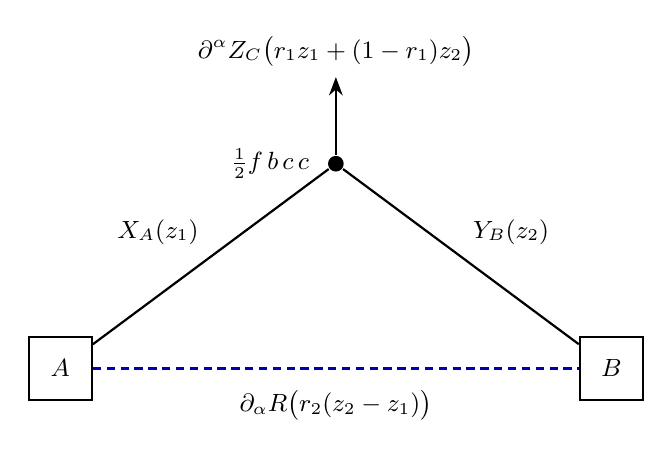
\begin{tikzpicture}[>=Stealth,thick,font=\small]
\node[draw,minimum size=8mm] (A) at (0,0) {$A$};
\node[draw,minimum size=8mm] (B) at (7,0) {$B$};
\node[circle,fill,inner sep=2pt] (I) at (3.5,2.6) {};
\node[left=6pt] at (I) {$\tfrac12f\,b\,c\,c$};
\draw (A) -- node[above left=1pt]{$X_A(z_1)$} (I);
\draw (B) -- node[above right=1pt]{$Y_B(z_2)$} (I);
\draw[->] (I) -- ++(0,1.1) node[above]{$\partial^\alpha Z_C\big(r_1z_1+(1-r_1)z_2\big)$};
\draw[blue!70!black,densely dashed] (A) -- (B);
\node[below] at (3.5,-0.15) {$\partial_\alpha R\big(r_2(z_2-z_1)\big)$};
\end{tikzpicture}
\caption{The one-loop term of $A\star B$. The letters $X$ of $A$ and $Y$ of $B$, displaced by $z_1$ and $z_2$, are contracted with the interaction vertex; its third leg is the output letter $Z$. The dashed edge is the marked edge of the product; the remainder $R$ of $A$ is translated along it and differentiated once. The parameters $(r_1,r_2)$ run over the simplex of \eqref{eq-oneloop}.}
\label{fig-triangle}
\end{figure}

\begin{proposition}[One-loop product in letters]\label{prop-oneloop}
Let $A=R\,X_A(z_1)$ and $B=Y_B(z_2)\,R'$, where $X,Y\in\{b,c\}$ are letters displaced by $z_1,z_2$ from the insertion point, so that $\partial^mX_A=\partial_{z_1}^mX_A(z_1)|_{z_1=0}$ and likewise for $Y$. The contraction of $X$ with $Y$ contributes to $[\hbar](A\star B)$ the term
\begin{equation}\label{eq-oneloop}
f_{ABC}\int_0^1\!dr_1\int_0^{1-r_1}\!dr_2\ \,
\partial_\alpha R\big(r_2(z_2-z_1)\big)\ \partial^\alpha Z_C\big(r_1z_1+(1-r_1)z_2\big)\ R',
\end{equation}
where $R(y)$ is $R$ translated by $y$, and $Z=c$ for $(X,Y)=(b,c)$ or $(c,b)$, $Z=b$ for $(X,Y)=(b,b)$; the pair $(c,c)$ does not contribute. $[\hbar](A\star B)$ is the sum of these terms over all pairs of letters, with the sign of bringing $X$ to the right end of $A$ and $Y$ to the left end of $B$. Without derivatives on $X$ and $Y$,
\begin{equation}\label{eq-oneloop-zero}
[\hbar]\big(R\,X_A\star Y_B\,R'\big)\ \ni\ \tfrac12\,f_{ABC}\ \partial_\alpha R\ \partial^\alpha Z_C\ R' .
\end{equation}
\end{proposition}

\begin{proofbox}
The triangle with vertices $\mathcal I$, $A$, $B$ and marked edge $(A,B)$ has the kernel of \cite[Equation~(6.28)]{LLCh}: the surviving field of the interaction is evaluated at $r_1z_1+(1-r_1)z_2$ with one derivative, the uncontracted part of $A$ is translated by $r_2(z_2-z_1)$ and differentiated once, and $(r_1,r_2)$ is integrated over $0\le r_1$, $0\le r_2$, $r_1+r_2\le1$. For the interaction $\tfrac12f_{ABC}b_Ac_Bc_C$ the contracted pairs and the output letter are as stated. The overall constants of the three channels are fixed by Theorem~\ref{thm-LLCh}(i) at order $\hbar$,
\begin{equation}\label{eq-leibniz1}
\begin{aligned}
&Q_0\,[\hbar](A\star B)-[\hbar]\big((Q_0A)\star B\big)-(-1)^{|A|}[\hbar]\big(A\star(Q_0B)\big)\\
&\qquad=-\Big(Q_1(AB)-(Q_1A)B-(-1)^{|A|}A\,(Q_1B)\Big),
\end{aligned}
\end{equation}
evaluated on single letters with the normalisation \eqref{eq-Q1}; the identity \eqref{eq-leibniz1} then holds on all products of letters (Appendix~\ref{app-ranks}).
\end{proofbox}

The derivative in \eqref{eq-oneloop} acts on the whole remainder of $A$. For this reason the one-loop correction of multiplication by an operator that contains $b$ is not a derivation of single letters. Multiplication by $C_0$, which contains no $b$, is simpler.

\begin{corollary}[Multiplication by the gaugino bilinear]\label{cor-L}
The operator $L=C_0\star{}$ commutes with $\Qp$ and has the expansion
\begin{equation}\label{eq-L}
L=C_0\cdot{}+\hbar\,\theta+\hbar^2L^{(2)}+\cdots,
\end{equation}
in which the term of order $\hbar^n$ contracts $n$ letters $b$ of the operator it acts on and vanishes on operators with fewer than $n$ of them. The one-loop term $\theta$ is the derivation with $\theta(\partial^mc_A)=0$ and
\begin{equation}\label{eq-theta}
\theta(b_A)=-\tfrac13\,f_{ABC}\,\partial_\alpha\partial_\beta c_B\,\partial^\alpha\partial^\beta c_C ,
\end{equation}
and its values on $\partial^mb_A$ follow from \eqref{eq-oneloop}. The first two orders of $[\Qp,L]=0$ are
\begin{equation}\label{eq-L-eqs}
[Q_0,\theta]=-[Q_1,C_0\,\cdot\,],\qquad [Q_0,L^{(2)}]=-[Q_1,\theta]-[Q_2,C_0\,\cdot\,].
\end{equation}
\end{corollary}

\begin{proofbox}
$[\Qp,L]=0$ is Theorem~\ref{thm-LLCh}(i) with $\Qp C_0=0$. A graph of order $\hbar^n$ has $2n$ contractions, each joining a letter $b$ to a letter $c$; the interaction vertices supply $n$ letters $b$ and $C_0$ none, so $n$ letters $b$ of the second factor are contracted. At order $\hbar$ the single vertex contracts its $b$-leg with a letter of $C_0$ and one $c$-leg with a letter $b$, so $\theta$ is a derivation that acts on the letters $b$. For \eqref{eq-theta}, apply \eqref{eq-oneloop} to $X=\partial_\gamma c_D$ in $C_0$ and $Y=b_A$: differentiating once in $z_1$ gives $\int r_1=\int r_2=\tfrac16$ over the simplex, the term with $\partial_\gamma\partial_\alpha\partial^\gamma c$ vanishes, and the two letters of $C_0$ contribute equally. The result solves the first equation of \eqref{eq-L-eqs} on $b_A$.
\end{proofbox}

Since the output letter of \eqref{eq-oneloop} sits at $r_1z_1+(1-r_1)z_2$ rather than at the position of $b$, the derivation $\theta$ does not commute with $\partial_\alpha$: $\theta(\partial_\alpha b_A)\neq\partial_\alpha\theta(b_A)$.

\subsection{Two loops and beyond}\label{sec-product-twoloop}

At order $\hbar^n$ the product is the graph sum of \cite[Equation~(6.26)]{LLCh}, which reduces to the product forests of \cite[Section~7]{LLCh}. Each connected component of a forest is a full binary rooted tree: its internal vertices are interaction vertices, its leaves are contractions with letters of $A$ or of $B$, and its root keeps one uncontracted leg, the letter that the tree produces. A forest $F$ carries a kernel, a polynomial in the derivatives that act on the produced letters and on the remainder of $A$; its Taylor coefficients in the displacements of the contracted letters give the action on letters with derivatives. The term $[\hbar^n](A\star B)$ is the sum over the forests with $n$ interaction vertices, weighted by the inverse order of their automorphism groups, and over the assignments of letters of $A$ and $B$ to the leaves. Its normalisation is the $n$-th power of the one-loop normalisation of Proposition~\ref{prop-oneloop}, so that no constant is free beyond one loop.

For $n=1$ the only forest is the triangle of Figure~\ref{fig-triangle}. For $n=2$ there are three \cite[Equation~(6.29) and Figure~6.3]{LLCh}. The first consists of two triangles: two letters of $A$ and two letters of $B$ are contracted pairwise through the two interaction vertices. Without derivatives on the contracted letters its kernel is \cite[Equation~(6.30)]{LLCh}
\begin{equation}\label{eq-book}
\begin{aligned}
&\tfrac1{24}\,\langle q_1,q_2+2p\rangle\,\langle q_2,q_1+2p\rangle\\
&\qquad=\tfrac16\langle p,q_1\rangle\langle p,q_2\rangle+\tfrac1{12}\langle q_1,q_2\rangle\big(\langle p,q_1\rangle-\langle p,q_2\rangle\big)-\tfrac1{24}\langle q_1,q_2\rangle^2,
\qquad \langle p,q\rangle=\epsilon^{\alpha\beta}p_\alpha q_\beta,
\end{aligned}
\end{equation}
where $p$ is the derivative acting on the remainder of $A$ and $q_1,q_2$ are the derivatives acting on the two produced letters. The other two forests are single trees: one interaction vertex is joined to $A$, to $B$ and to the second vertex, and the second vertex is joined to $A$, respectively to $B$, and produces the output letter. Two letters of one operator and one letter of the other are contracted, and the kernel without derivatives is $-\tfrac1{24}\langle q,p\rangle^2$, respectively $+\tfrac1{24}\langle q,p\rangle^2$. The kernels for contracted letters with derivatives are those of \cite[Equations~(6.31)--(6.33)]{LLCh}. This gives $[\hbar^2](A\star B)$ for all letters with arbitrary derivatives, and Theorem~\ref{thm-LLCh}(i) at this order reads
\begin{equation}\label{eq-leibniz2}
\sum_{i+j=2}\Big(Q_i\,[\hbar^j](A\star B)-[\hbar^j]\big((Q_iA)\star B\big)-(-1)^{|A|}[\hbar^j]\big(A\star(Q_iB)\big)\Big)=0 .
\end{equation}
With $A=C_0$ the two-loop term is the operator $L^{(2)}$ of \eqref{eq-L}, of second order in the letters $b$.

The corrections $Q_n$ of the supercharge are sums of fan graphs, whose kernels are known in closed form at every loop order \cite[Section~5]{LLCh}. The product involves more graphs: there are $1,3,8,23,65,194$ forests for $n=1,\dots,6$, and their kernels are evaluated graph by graph \cite[Section~7]{LLCh}.

\section{Lifts forced by the gaugino bilinear}\label{sec-mechanism}

\subsection{The primitive of $C_0^N$ and the homotopy}\label{sec-homotopy}

In $\Ep$ the $N$-th power of $C_0$ vanishes: there is an operator $x_N\in V$ without letters $b$ such that
\begin{equation}\label{eq-xN}
Q_0\,x_N=C_0^N,\qquad Q_n\,x_N=0\quad(n\ge1).
\end{equation}
For $SU(2)$,
\begin{equation}\label{eq-x2}
x_2=-\tfrac23\,f_{ABC}\,\partial_\alpha c_A\,\partial_\beta c_B\,\partial^\alpha\partial^\beta c_C .
\end{equation}
The operator $x_N$ has $N_c=2N-1$ and lies at $(N,N)$, so by \eqref{eq-selection} $\Qi\,x_N$ has $N_c=0$ at $(0,0)$: it is a number. The exact theory enters through the following hypothesis.

\begin{assumption}[Exact product]\label{ass-exact}
There is an odd operator $h$ on $V[[\Lambda^{3N}]]$, equal to multiplication by $x_N$ at order $\hbar^0\Lambda^0$, and an even operator $L$, equal to $C_0\star{}$ at order $\Lambda^0$, such that
\begin{equation}\label{eq-homotopy}
[Q,L]=0,\qquad Qh+hQ=L^N-\nu\,\Lambda^{3N},\qquad \nu\neq0 .
\end{equation}
\end{assumption}

\begin{remark}[Origin of the assumption]\label{rem-origin}
Suppose that the exact theory has a product of local operators that reduces to $\star$ at order $\Lambda^0$, for which $Q$ is a derivation, and whose multiplication operators compose up to $Q$-homotopy, as in Theorem~\ref{thm-LLCh}(i) and (iii). Let $L$ be the multiplication by $C_0$. The relation $[C_0]^N=\nu\Lambda^{3N}$ of the infrared theory \cite{VY} states that the $N$-fold product of $C_0$ minus $\nu\Lambda^{3N}$ is $Q$-exact, with a primitive that reduces to $x_N$ by \eqref{eq-xN}. Since this primitive is odd, the Leibniz rule gives $\{Q,x_N\star{}\}=(Qx_N)\star{}$, and subtracting the homotopy between the multiplication by an $N$-fold product and $L^N$ gives $h$. At order $\Lambda^0$ and $\hbar^1$, \eqref{eq-homotopy} reads
\begin{equation}\label{eq-eta}
h=x_N\cdot{}+\hbar\,\eta+\cdots,\qquad \{Q_0,\eta\}=N\,C_0^{N-1}\theta-\{Q_1,x_N\,\cdot\,\},
\end{equation}
an equation for an odd derivation $\eta$ of the letters $b$, which we solve explicitly in Section~\ref{sec-partners}.
\end{remark}

\subsection{The triple product and the main theorem}\label{sec-theorem}

\begin{definition}[Triple product]\label{def-triple}
Let $a\in\Ep$ with $C_0\,a=0$ in $\Ep$: for a cocycle of $\Qp$ representing $a$, again denoted $a$, there is $w\in V$ with $\Qp w=L\,a$. Then
\begin{equation}\label{eq-triple}
\langle C_0^{N-1},C_0,a\rangle:=\big[\,h\,a-L^{N-1}w\,\big]\ \in\ \Ep\big/C_0^{N-1}\Ep ,
\end{equation}
where $h$ and $L$ are taken at order $\Lambda^0$.
\end{definition}

\begin{lemma}\label{lem-triple}
The element $h\,a-L^{N-1}w$ is a cocycle of $\Qp$, and its class modulo $C_0^{N-1}\Ep$ depends only on the class $a$. It lies at $(n_1+N,n_2+N)$ with $N_c+2N-1$ letters $c$ if $a$ lies at $(n_1,n_2)$ with $N_c$.
\end{lemma}

\begin{proofbox}
At order $\Lambda^0$, \eqref{eq-homotopy} gives $\Qp h+h\Qp=L^N$ and $[\Qp,L]=0$. Hence
\[
\Qp\big(h\,a-L^{N-1}w\big)=\underbrace{L^Na-h\,\Qp a}_{\Qp(ha)}-\underbrace{L^{N-1}L\,a}_{L^{N-1}\Qp w}=0 .
\]
Replacing $w$ by $w+y$ with $\Qp y=0$ changes the element by $-L^{N-1}y$, whose class is in $C_0^{N-1}\Ep$. Replacing $a$ by $a+\Qp u$ and $w$ by $w+Lu$ changes it by $h\,\Qp u-L^Nu=-\Qp(hu)$. The degrees are those of $x_N\,a$.
\end{proofbox}

The degree shift in Lemma~\ref{lem-triple} is the opposite of the selection rule \eqref{eq-selection}. The construction is a Massey triple product \cite{Massey}: $C_0^{N-1}\cdot C_0$ and $C_0\cdot a$ both vanish in $\Ep$, with primitives $x_N$ and $w$.

\begin{theorem}[The instanton inverts the triple product]\label{thm-mechanism}
Under Assumption~\ref{ass-exact}, for every $a\in\Ep$ with $C_0\,a=0$, the class $\Qi\,a$ is annihilated by $C_0$, and
\begin{equation}\label{eq-mechanism}
\Qi\,\langle C_0^{N-1},C_0,a\rangle+\langle C_0^{N-1},C_0,\Qi\,a\rangle=-\nu\,a
\qquad\text{in}\quad \Ep\big/C_0^{N-1}\Ep .
\end{equation}
\end{theorem}

\begin{proofbox}
Choose $\tilde a$ as in Definition~\ref{def-Qi}, so that $Q\tilde a=\Lambda^{3N}e+O(\Lambda^{6N})$ with $e$ representing $\Qi\,a$. Since $L\tilde a$ reduces to $\Qp w$ at order $\Lambda^0$, there are $\tilde w$, reducing to $w$, and $u$ with
\[
L\,\tilde a=Q\tilde w+\Lambda^{3N}u+O(\Lambda^{6N}).
\]
Applying $Q$ and using $[Q,L]=0$ gives $\Qp u=L\,e$ at order $\Lambda^{3N}$: the class $\Qi\,a$ is annihilated by $C_0$, and $u$ is a primitive for it. Then, by \eqref{eq-homotopy},
\begin{align*}
Q\big(h\,\tilde a-L^{N-1}\tilde w\big)
&=\underbrace{\big(L^N-\nu\Lambda^{3N}\big)\tilde a-h\,Q\tilde a}_{Q(h\tilde a)}-\underbrace{L^{N-1}\big(L\tilde a-\Lambda^{3N}u\big)}_{L^{N-1}Q\tilde w}+O(\Lambda^{6N})\\
&=-\Lambda^{3N}\Big(\nu\,\tilde a+h\,e-L^{N-1}u\Big)+O(\Lambda^{6N}).
\end{align*}
The term of order $\Lambda^0$ of $h\tilde a-L^{N-1}\tilde w$ represents $\langle C_0^{N-1},C_0,a\rangle$, so by Definition~\ref{def-Qi} the left side computes $\Lambda^{3N}\,\Qi\langle C_0^{N-1},C_0,a\rangle$; on the right, $h\,e-L^{N-1}u$ represents $\langle C_0^{N-1},C_0,\Qi\,a\rangle$. The ambiguity of the triple products is in $C_0^{N-1}\Ep$, which $\Qi$ preserves because it commutes with $L$ on $\Ep$.
\end{proofbox}

\begin{corollary}[Forced partners]\label{cor-forced}
Let $a\in\Ep$ satisfy $C_0\,a=0$ and $\Qi\,a=0$, and suppose that $a\notin C_0^{N-1}\Ep$. Then $\langle C_0^{N-1},C_0,a\rangle\neq0$ and
\begin{equation}\label{eq-forced}
\Qi\,\langle C_0^{N-1},C_0,a\rangle=-\nu\,a\quad\text{modulo}\ \ C_0^{N-1}\Ep .
\end{equation}
In particular every class annihilated by both $C_0$ and $\Qi$ is $\Qi$-exact modulo $C_0^{N-1}\Ep$.
\end{corollary}

\begin{remark}[The relation itself]\label{rem-extension}
The element $x_N$ is not a cocycle of $\Qp$, so $[C_0]^N=\nu\Lambda^{3N}$ is not a value of $\Qi$ on $\Ep$. It is a multiplicative extension: on $\Ep$ the product $C_0^N$ vanishes, and in the exact cohomology it equals $\nu\Lambda^{3N}$. Theorem~\ref{thm-mechanism} is what this extension implies for the differential.
\end{remark}

\section{Explicit partners}\label{sec-partners}

In the examples below the leading component of $h\,a-L^{N-1}w$ is $Q_0$-exact, and the class is represented one loop order lower. Its computation therefore needs the corrections $\theta$, $\eta$ and $L^{(2)}$ of Section~\ref{sec-product} together with $Q_1$, $Q_2$ and $Q_3$.

\subsection{$SU(2)$: the partner of $C_2$}\label{sec-C2}

The class $C_2$ at $(3,3)$ has the cocycle
\begin{equation}\label{eq-C2}
a=a_2+\hbar\,a_1+\hbar^2a_0,\qquad a_2=-\tfrac12\,b_Ab_A\,C_0,\qquad Q_0a_1=-Q_1a_2,\quad Q_0a_0=-Q_1a_1-Q_2a_2 .
\end{equation}
The product $C_0\,a$ lies at $(4,4)$ with $N_c=4$, where $\Ep=0$ (Table~\ref{tab-census}); hence $C_0\,C_2=0$, and $\Qi\,C_2=0$ because its target at $(1,1)$ with $N_c=-1$ is empty. Corollary~\ref{cor-forced} applies and predicts a nonzero class at $(5,5)$ with $N_c=5$.

\begin{proposition}[Partner of $C_2$]\label{prop-C2}
Let $w=w_2+\hbar w_1+\hbar^2w_0$ solve $\Qp w=L\,a$ and let $n_2$ solve $Q_0n_2=x_2a_2-C_0w_2$. Then
\begin{equation}\label{eq-m1}
\langle C_0,C_0,C_2\rangle=\hbar\,\big[\,x_2a_1+\eta(a_2)-C_0w_1-\theta(w_2)-Q_1n_2\,\big],
\end{equation}
and this is $\hbar$ times a nonzero element of the one-dimensional space $\Ep$ at $(5,5)$, $(N_b,N_c)=(1,5)$. Consequently
\begin{equation}\label{eq-C2-lift}
\Qi\,\langle C_0,C_0,C_2\rangle=-\nu\,C_2 .
\end{equation}
\end{proposition}

\begin{proofbox}
With \eqref{eq-L} and \eqref{eq-eta},
\[
h\,a-L\,w=\underbrace{x_2a_2-C_0w_2}_{N_b=2:\ \ =Q_0n_2}+\hbar\,\underbrace{\big(x_2a_1+\eta(a_2)-C_0w_1-\theta(w_2)\big)}_{N_b=1}+O(\hbar^2),
\]
and subtracting $\Qp n_2$ gives \eqref{eq-m1}. The operators are computed as follows. The derivation $\theta$ is given by Corollary~\ref{cor-L}. The equation \eqref{eq-eta} for $\eta$, an odd derivation $b_A\mapsto\eta_A$, has a unique solution, and so has \eqref{eq-L-eqs} for $L^{(2)}$, a second-order operator $b_Ab_B\mapsto\lambda_{AB}$. The component $w_1$ is determined by $Q_0w_1=C_0a_1+\theta(a_2)-Q_1w_2$ up to the classes of $E_1$ at $(4,4)$, $(N_b,N_c)=(1,3)$, a two-dimensional space whose multiples by $C_0$ are nonzero in $E_1$ at $(5,5)$, $(1,5)$. This freedom is fixed by the component $N_b=0$ of $\Qp w=L\,a$, which contains $Q_2$ and $L^{(2)}$: the triple product is a two-loop quantity. With the solution, the class of \eqref{eq-m1} in the one-dimensional space $E_1$ at $(5,5)$, $(1,5)$ is nonzero; this space has $d_1=0$ and no incoming or outgoing higher differential, so it equals $\Ep$ there. All steps are carried out with rational coefficients, and three further choices of the representatives $a_1$, $w_2$, $w_1$ give the same class. Since $\Ep$ vanishes at $(2,2)$ and at $(4,4)$, the space $C_0\Ep$ is zero in the degrees of $C_2$ and of its partner, and \eqref{eq-C2-lift} is \eqref{eq-forced}.
\end{proofbox}

The partner is the class $(1,5)$ at $(5,5)$ of Table~\ref{tab-census}, which \cite[Table~3]{semichiral} writes as $B_{1,2}\,\partial_2C_0\,\partial_1^2C_0$. Its restriction to the Cartan subalgebra, where $b$ and $c$ have one component each, is a nonzero multiple of
\begin{equation}\label{eq-J}
b\,J,\qquad J:=\partial_2c\ \partial_2^2c\ \partial_1c\ \partial_1\partial_2c\ \partial_1^2c .
\end{equation}

\subsection{$SU(3)$: the partner of $C_1$}\label{sec-C1}

For $SU(3)$ the class $C_1$ at $(2,2)$ has a cocycle with a single component, $a=a_1$ with $Q_1a_1=0$, and $C_0\,C_1$ lies at $(3,3)$, where $\Ep=0$. Now $N=3$: with $Q_0x_3=C_0^3$,
\begin{equation}\label{eq-su3-ops}
L^2=C_0^2\cdot{}+2\hbar\,C_0\,\theta+\cdots,\qquad h=x_3\cdot{}+\hbar\,\eta+\cdots,\qquad \{Q_0,\eta\}=3\,C_0^2\,\theta-\{Q_1,x_3\,\cdot\,\},
\end{equation}
and one loop suffices because $a$ has $N_b=1$.

\begin{proposition}[Partner of $C_1$]\label{prop-C1}
Let $w=w_1+\hbar w_0$ solve $\Qp w=L\,a$ and let $Q_0n_1=x_3a_1-C_0^2w_1$. Then
\begin{equation}\label{eq-su3-m0}
\langle C_0^2,C_0,C_1\rangle=\hbar\,\big[\,\eta(a_1)-C_0^2w_0-2\,C_0\,\theta(w_1)-Q_1n_1\,\big]
\end{equation}
is $\hbar$ times a nonzero class of $\Ep$ at $(5,5)$, $(N_b,N_c)=(0,7)$, and $\Qi\,\langle C_0^2,C_0,C_1\rangle=-\nu\,C_1$.
\end{proposition}

\begin{proofbox}
The expansion of $h\,a-L^2w$ is $\big(x_3a_1-C_0^2w_1\big)+\hbar\big(\eta(a_1)-C_0^2w_0-2C_0\theta(w_1)\big)$, which gives \eqref{eq-su3-m0}. To see that the class is nonzero we restrict all letters to the Cartan subalgebra. By \eqref{eq-Q0} the restriction of every $Q_0$-exact operator vanishes. With $c_1,c_2$ the two Cartan components of $c$, the restriction of the representative in \eqref{eq-su3-m0} is
\begin{equation}\label{eq-su3-cartan}
40\ \partial_1c_1\,\partial_2c_1\,\partial_1c_2\,\partial_2c_2\!\!\sum_{\substack{(i,j,k)\in\{1,2\}^3\\ \text{not all equal}}}\!\!\pm\ \partial_1^2c_i\ \partial_1\partial_2c_j\ \partial_2^2c_k\ \neq0 ,
\end{equation}
unchanged under the remaining freedom in $w_1$ and in $\eta$. The representative is therefore not $Q_0$-exact, and since $d_1$ from $(N_b,N_c)=(1,6)$ to $(0,7)$ has rank zero at $(5,5)$, it is nonzero in $\Ep$. The target of $\Qi\,C_1$ is empty and $C_0^2\Ep$ vanishes at $(2,2)$, $N_c=2$, so Corollary~\ref{cor-forced} gives the last statement. The coefficients are computed modulo $2^{31}-1$.
\end{proofbox}

This is the class $(0,7)$ at $(5,5)$ of Table~\ref{tab-census}, in the sector that \cite[Section~8]{semichiral} identified as the place of the partner of $C_1$.

\subsection{The $SU(2)$ tower: hidden products and matric triple products}\label{sec-tower}

The classes $C_4$ at $(5,5)$ and $C_6$ at $(7,7)$ have cocycles
\begin{equation}\label{eq-C4}
C_4=a_4+\hbar\,a_3+\hbar^2(C_4)_{N_b=2}+\cdots,\qquad C_6=a_6+\hbar\,a_5+\cdots,
\end{equation}
which we construct through $Q_3$; the leading components are proportional to $(b_Ab_A)^2C_0$ and $(b_Ab_A)^3C_0$, and we normalise them by $C_0\,a_4=a_2^2$ and $C_0\,a_6=a_2a_4$. Their products with $C_0$ are not zero.

\begin{proposition}[Hidden products]\label{prop-hidden}
In $\Ep$ for $SU(2)$:
\begin{enumerate}
\item[(i)] $C_0\,C_4$ is a nonzero multiple of the class at $(6,6)$, and $C_0\,C_6$ a nonzero multiple of the class $(4,4)$ at $(8,8)$;
\item[(ii)] $C_2^2=-3\,C_0\,C_4$ and $C_2\,C_4=-\tfrac53\,C_0\,C_6$.
\end{enumerate}
\end{proposition}

\begin{proofbox}
For (i), expand $L\,C_4$ with \eqref{eq-L}. The components with $N_b=4$ and $N_b=3$ are removed by exact terms, $C_0a_4=Q_0k_4$ and $C_0a_3+\theta(a_4)-Q_1k_4=Q_0k_3$, leaving at order $\hbar^2$
\[
r_2=C_0\,(C_4)_{N_b=2}+\theta(a_3)+L^{(2)}(a_4)-Q_2k_4-Q_1k_3 ,
\]
which is $Q_0$-closed and $d_1$-closed. It is not in the sum of the image of $Q_0$ and the image of $d_1$ at $(6,6)$, $(N_b,N_c)=(2,4)$, and its Cartan restriction is not in the restriction of the image of $d_1$; three independent choices of $(C_4)_{N_b=2}$ agree. The same computation at $(8,8)$ gives $C_0C_6\neq0$. For (ii), the product $C_2\star C_2$ is expanded with the one- and two-loop terms of Section~\ref{sec-product}:
\begin{align*}
C_2\star C_2={}&\underbrace{a_2^2}_{=Q_0k_4}+\hbar\,\underbrace{\big(2a_1a_2+[\hbar](a_2\star a_2)\big)}_{=Q_1k_4+Q_0k_3}\\
&+\hbar^2\big(2a_0a_2+a_1^2+[\hbar](a_2\star a_1+a_1\star a_2)+[\hbar^2](a_2\star a_2)\big)+\cdots,
\end{align*}
and the component of order $\hbar^2$, reduced as before, equals $-3$ times that of $C_0\star C_4$ modulo the images of $Q_0$ and $d_1$. The second relation is obtained in the same way at $(8,8)$. Coefficients are modulo $2^{31}-1$.
\end{proofbox}

By Proposition~\ref{prop-hidden}(i) the classes $C_4$ and $C_6$ are not annihilated by $C_0$, and Definition~\ref{def-triple} does not apply to them. The relations (ii) provide the replacement. In the rest of this subsection the gauge group is $SU(2)$ and $N$ denotes the operator $C_2\star{}$. Let $w$ be as in Proposition~\ref{prop-C2}, and let $v$ and an odd operator $\kappa$ satisfy
\begin{equation}\label{eq-v-kappa}
\Qp v=L\,C_4+\tfrac13\,N\,C_2,\qquad \{\Qp,\kappa\}=LN-NL ;
\end{equation}
$v$ exists by Proposition~\ref{prop-hidden}(ii). By Theorem~\ref{thm-LLCh}(iii) there is an element $e$ with $\Qp e=C_0\star C_2-C_2\star C_0$, and $\kappa$ is the corresponding homotopy between the two orders of multiplication, with leading term the multiplication by $e$.

\begin{proposition}[Partner of $C_4$]\label{prop-M4}
The element
\begin{equation}\label{eq-M4}
M_4=h\,C_4-L\,v+\tfrac13\big(N\,w+\kappa\,C_2\big)
\end{equation}
is a cocycle of $\Qp$. It represents the class $(3,5)$ at $(7,7)$ of Table~\ref{tab-census}, and under Assumption~\ref{ass-exact}, with an exact product as in Remark~\ref{rem-origin},
\begin{equation}\label{eq-M4-lift}
\Qi\,M_4=-\nu\,C_4 .
\end{equation}
\end{proposition}

\begin{proofbox}
Using $\{\Qp,h\}=L^2$, $[\Qp,L]=[\Qp,N]=0$ and \eqref{eq-v-kappa},
\[
\Qp M_4=\underbrace{L^2C_4}_{\Qp(hC_4)}-\underbrace{L\big(LC_4+\tfrac13NC_2\big)}_{L\,\Qp v}+\tfrac13\Big(\underbrace{N\,L\,C_2}_{N\,\Qp w}+\underbrace{(LN-NL)\,C_2}_{\{\Qp,\kappa\}C_2}\Big)=0 .
\]
The order of the factors matters: with the product $\star$ alone, the combination $x_2\star C_4+\tfrac13w\star C_2-C_0\star v$ fails to be closed at the first corrected order, because $\star$ is associative and commutative only up to exact terms; $\eta$ and $\kappa$ supply them. The leading component of $M_4$ is $Q_0$-exact, $x_2a_4-C_0v_4+\tfrac13a_2w_2=Q_0n_4$, and the next component, minus $Q_1n_4$, restricts on the Cartan subalgebra to a nonzero multiple of $b^3J$, with $J$ as in \eqref{eq-J}. At $(7,7)$, $E_1$ vanishes at $(N_b,N_c)=(4,5)$ and is one-dimensional at $(3,5)$ with no incoming $d_1$, so $M_4$ is the class of the table. For \eqref{eq-M4-lift}, repeat the proof of Theorem~\ref{thm-mechanism} with the exact operators $L$, $N$, $h$ and $\kappa$, for which $\{Q,\kappa\}=LN-NL$ and \eqref{eq-homotopy} hold. The cocycle conditions of $C_2$ and $C_4$ and the two relations $\Qp w=L\,C_2$ and $\Qp v=L\,C_4+\tfrac13N\,C_2$ acquire corrections of order $\Lambda^6$, which are cocycles of $\Qp$ at $(1,1)$ and $(3,3)$ with $N_c=-1$ and at $(2,2)$ and $(4,4)$ with $N_c=0$; there are no operators, respectively no classes, in these degrees (Table~\ref{tab-census}), so the corrections are exact and are absorbed in $w$ and $v$. The only remaining term of order $\Lambda^6$ is $-\nu\,C_4$ from \eqref{eq-homotopy}.
\end{proofbox}

The partner of $C_6$ is constructed in the same way. With $N_4=C_4\star{}$ and elements $v$, $e_{04}$, $e_{24}$ such that
\begin{equation}\label{eq-M6-inputs}
\Qp v=L\,C_6+\tfrac35\,C_2\star C_4,\qquad \Qp e_{04}=C_0\star C_4-C_4\star C_0,\qquad \Qp e_{24}=C_2\star C_4-C_4\star C_2,
\end{equation}
the element
\begin{equation}\label{eq-M6}
M_6=h\,C_6-L\,v+\tfrac35\big(N_4\,w+e_{04}\,C_2+L\,e_{24}\big)
\end{equation}
is closed in its two leading components, its Cartan restriction is a nonzero multiple of $b^5J$, and it represents the class $(5,5)$ at $(9,9)$; as in Proposition~\ref{prop-M4}, $\Qi\,M_6=-\nu\,C_6$.

Figure~\ref{fig-pairs} collects the pairs. The two remaining classes of Table~\ref{tab-census} are multiples of these by $C_0$.

\begin{corollary}[Multiples by $C_0$]\label{cor-multiples}
Under Assumption~\ref{ass-exact}, $\Qi(C_0\,M_4)=-\nu\,C_0\,C_4\neq0$ and $\Qi(C_0\,M_6)=-\nu\,C_0\,C_6\neq0$. Hence $C_0\,M_4$ is a nonzero multiple of the class $(1,7)$ at $(8,8)$, and $C_0\,M_6$ is a nonzero class at $(10,10)$ with $N_c=7$.
\end{corollary}

\begin{proofbox}
$\Qi$ commutes with $L$ on $\Ep$, by $[Q,L]=0$ at order $\Lambda^6$. The right sides are nonzero by Proposition~\ref{prop-hidden}(i), and $\Ep$ at $(8,8)$ with $N_c=7$ is one-dimensional.
\end{proofbox}

\begin{figure}[H]
\centering
\begin{tikzpicture}[>=Stealth,x=1.15cm,y=0.72cm,font=\small]
\draw[->,gray] (-0.4,0) -- (10.9,0) node[right,black]{$n$};
\draw[->,gray] (0,-0.4) -- (0,8.2) node[above,black]{$N_c$};
\foreach \x in {1,...,10} \draw[gray] (\x,0.08)--(\x,-0.08) node[below,black]{\footnotesize\x};
\foreach \y in {2,4,5,7} \draw[gray] (0.06,\y)--(-0.06,\y) node[left,black]{\footnotesize\y};
\tikzset{cl/.style={circle,fill=black,inner sep=1.6pt},pr/.style={circle,draw=black,fill=white,inner sep=1.6pt}}
\node[cl,label=above right:{$1$}] at (0,0) {};
\node[cl,label=above:{$C_0$}] at (1,2) {};
\node[cl,label=below:{$C_2$}] (c2) at (3,2) {};
\node[cl,label=below:{$C_4$}] (c4) at (5,2) {};
\node[cl,label=below:{$C_6$}] (c6) at (7,2) {};
\node[cl,label=below right:{$C_0C_4$}] (c04) at (6,4) {};
\node[cl,label=below right:{$C_0C_6$}] (c06) at (8,4) {};
\node[cl,label=above left:{$\langle C_0,C_0,C_2\rangle$}] (t2) at (5,5) {};
\node[cl,label=right:{$M_4$}] (m4) at (7,5) {};
\node[cl,label=right:{$M_6$}] (m6) at (9,5) {};
\node[cl,label=above:{$C_0M_4$}] (m04) at (8,7) {};
\node[pr,label=above:{$C_0M_6$}] (m06) at (10,7) {};
\draw[->,blue!70!black] (t2) -- (c2);
\draw[->,blue!70!black] (m4) -- (c4);
\draw[->,blue!70!black] (m6) -- (c6);
\draw[->,blue!70!black] (m04) -- (c04);
\draw[->,blue!70!black] (m06) -- (c06);
\end{tikzpicture}
\caption{Perturbative classes of $SU(2)$ at $(n,n)$ with $N_c$ letters $c$, and the action of $\Qi$ (arrows), each equal to $-\nu$ times the class at its tip. Filled dots are classes of Table~\ref{tab-census}; the open dot is the class of Corollary~\ref{cor-multiples} beyond the computed range.}
\label{fig-pairs}
\end{figure}

The relations of Proposition~\ref{prop-hidden} take a uniform shape in the normalisation
\begin{equation}\label{eq-Dj}
D_0=-C_0,\qquad D_j=(2j-1)\,C_{2j}\quad(j\ge1):\qquad D_1D_1=D_0D_2,\qquad D_1D_2=D_0D_3 .
\end{equation}
In the exact cohomology they give a second derivation of the lifts, independent of the explicit partners.

\begin{corollary}[The tower in the exact ring]\label{cor-ring}
Under Assumption~\ref{ass-exact} and with an exact product as in Remark~\ref{rem-origin}, the classes of $C_2$, $C_4$ and $C_6$ vanish in the exact cohomology with $\Lambda$ inverted.
\end{corollary}

\begin{proofbox}
By \eqref{eq-C2-lift}, $[D_1]=0$. The relations \eqref{eq-Dj} hold in the exact ring: their corrections of order $\Lambda^6$ are cocycles at $(4,4)$ and at $(6,6)$ with $N_c=0$, where $\Ep$ vanishes. Then $[D_0][D_2]=[D_1]^2=0$ and $[D_0][D_3]=[D_1][D_2]=0$, and $[D_0]$ is invertible because $[D_0]^2=\nu\Lambda^6\neq0$.
\end{proofbox}

The Cartan restrictions of the three pairs follow one pattern. In a common normalisation, the ratio of the coefficient of $b^{2j-1}J$ in the partner of $C_{2j}$ to the coefficient of $b^{2j}\,\partial_2c\,\partial_1c$ in $C_{2j}$ is
\begin{equation}\label{eq-ratios}
-30,\quad -70,\quad -126\qquad(j=1,2,3),\qquad\text{that is}\quad -2\,(2j+1)(2j+3);
\end{equation}
the common factor depends on the normalisations of $C_0$ and of $\hbar$, the ratios $3\cdot5:5\cdot7:7\cdot9$ do not.

\section{The one-instanton input}\label{sec-instanton}

The constant $\nu$ is the value of the gaugino condensate \cite{NSVZ,VY}. We compute its one-instanton expression in the variables of the twisted theory for $SU(2)$, where $\partial_\alpha c_a$ is proportional to the gaugino $\bar\lambda_{\alpha a}$ \cite[Equation~(3.2)]{LLCh}, and locate the effect in the structure of Section~\ref{sec-mechanism}.

In the background of an instanton of size $\rho$ centred at $x_0$, with gauge orientation $R\in SO(3)$, the gaugino has four zero modes, two supersymmetric and two superconformal \cite{NSVZ,DHKMreview}:
\begin{equation}\label{eq-zm}
\bar\lambda^a_\alpha(y)=f(y)\,R^{ab}\,S^b_{\alpha\beta}\,\chi^\beta(y),\qquad
S^a=\sigma^a\epsilon,\qquad \chi^\beta(y)=\xi^\beta+y^{\beta\dot\gamma}\eta_{\dot\gamma},\qquad f(y)=\frac{\rho^2}{(y^2+\rho^2)^2},
\end{equation}
with $y=x-x_0$ and Grassmann parameters $\xi^\beta$, $\eta_{\dot\gamma}$.

\begin{lemma}[One point]\label{lem-onepoint}
On the zero modes \eqref{eq-zm}, with $W^c_{\alpha\beta}=\epsilon_{cab}\,\partial_\alpha c_a\,\partial_\beta c_b$,
\begin{equation}\label{eq-onepoint}
\partial_\alpha c_a\,\partial_\beta c_b=\tfrac16\,\delta_{ab}\,\epsilon_{\alpha\beta}\,C_0+\tfrac12\,\epsilon_{abc}\,W^c_{\alpha\beta},\qquad
W^c_{\alpha\beta}=\tfrac{i}{3}\,C_0\,R^{cd}S^d_{\alpha\beta},
\end{equation}
and $C_0^2=0$, $C_0\,W^c_{\alpha\beta}=0$ at one point.
\end{lemma}

\begin{proofbox}
At a point the zero modes depend on the two Grassmann variables $\chi^1(y),\chi^2(y)$ only. A product of two gauginos is proportional to $\chi^1\chi^2$, which gives \eqref{eq-onepoint} by the algebra of the matrices $S^a$; a product of three vanishes because $\chi^\alpha\chi^\beta\chi^\gamma=0$.
\end{proofbox}

The vanishing of $C_0^2$ at a point is the perturbative statement $C_0^2=Q_0x_2$: four zero modes cannot be absorbed by a single local operator built from two gaugino bilinears.

\begin{proposition}[Two points]\label{prop-twopoint}
For two insertions at $x_1\neq x_2$,
\begin{equation}\label{eq-twopoint}
\big\langle C_0(x_1)\,C_0(x_2)\big\rangle_{1\text{-inst}}=\mathcal N\,\frac{2\pi^2}{5}\,\Lambda^6 ,
\end{equation}
independent of $x_1-x_2$, where $\mathcal N$ is the normalisation of the collective-coordinate measure.
\end{proposition}

\begin{proofbox}
With $y_i=x_i-x_0$, the Grassmann integral is
\[
\int d^2\xi\,d^2\eta\ C_0(y_1)\,C_0(y_2)=36\,f(y_1)^2f(y_2)^2\,|x_1-x_2|^2 ,
\]
because $\chi^1\chi^2$ at $y_1$ times $\chi^1\chi^2$ at $y_2$ has top component $|y_1-y_2|^2$. The integral over the position and the size has the measure $d^4x_0\,d\rho\,\rho$, the power of $\rho$ being fixed by dimensional analysis once $\Lambda^6$ is factored out; it is evaluated with a Feynman parameter $\alpha$ and $r=x_1-x_2$:
\begin{align*}
\int d^4x_0\,\frac{1}{(y_1^2+\rho^2)^4(y_2^2+\rho^2)^4}&=\frac{10\pi^2}{3}\int_0^1d\alpha\ \frac{\alpha^3(1-\alpha)^3}{\big(\rho^2+\alpha(1-\alpha)r^2\big)^6},\\
\int_0^\infty d\rho\ \frac{\rho^9}{\big(\rho^2+\alpha(1-\alpha)r^2\big)^6}&=\frac{1}{10\,\alpha(1-\alpha)\,r^2},
\end{align*}
so that
\[
\int d^4x_0\,d\rho\ \rho\ \frac{\rho^8\,r^2}{(y_1^2+\rho^2)^4(y_2^2+\rho^2)^4}=\frac{\pi^2}{3}\int_0^1d\alpha\ \alpha^2(1-\alpha)^2=\frac{\pi^2}{90} .
\]
The factor $r^2$ cancels, and $36\cdot\pi^2/90=2\pi^2/5$.
\end{proofbox}

The independence of the separation is the cluster property used in \cite{NSVZ} to extract the condensate; the comparison of the resulting value with the one obtained at weak coupling is discussed in \cite{HKLM,DHKM}. For the present purpose \eqref{eq-twopoint} says that
\begin{equation}\label{eq-inst-product}
C_0\star C_0=\underbrace{C_0^2}_{=Q_0x_2}+\ \nu\,\Lambda^6\ \ \text{in the exact theory},\qquad \nu=\mathcal N\,\frac{2\pi^2}{5}:
\end{equation}
the leading instanton effect is a correction of the product of two operators, four zero modes shared as two and two between two points, and it has no counterpart on a single operator at this order of the semiclassical expansion. The identity \eqref{eq-homotopy} is \eqref{eq-inst-product} written for multiplication operators, and each lift of Section~\ref{sec-partners} uses it once: the partner and the class differ by $(n_1,n_2)=(2,2)$ and by three letters $c$, the charges of $x_2$. In the adjoint channel the same zero modes give $\langle W^c_{\alpha\beta}(x_1)\,W^d_{\gamma\delta}(x_2)\rangle=\tfrac{\nu\Lambda^6}{27}\,\delta^{cd}(\epsilon_{\alpha\gamma}\epsilon_{\beta\delta}+\epsilon_{\alpha\delta}\epsilon_{\beta\gamma})$.

\section{Massive matter}\label{sec-matter}

A chiral multiplet adds to the twisted theory an even field $\gamma$ and an odd field $\beta$ in conjugate representations, with $Q_0\beta=\partial W/\partial\gamma+c\cdot\beta$ and $Q_0\gamma=c\cdot\gamma$ \cite[Section~4]{semichiral}. A mass term is a quadratic superpotential and fixes the $R$-charge of $\gamma$ to one. We consider $SU(2)$ with
\begin{equation}\label{eq-theories}
\begin{array}{lll}
\text{(i)} & \text{no matter}; & \\
\text{(ii)} & \gamma_A\ \text{in the adjoint}, & W=m\,u,\quad u=\tfrac12\gamma_A\gamma_A;\\
\text{(iii)} & q,\ t\ \text{doublets}, & W=m\,M,\quad M=\epsilon_{ab}\,q^at^b .
\end{array}
\end{equation}
Below the mass the matter decouples and the theory is pure $SU(2)$ with scale $\Lambda_L$, $\Lambda_L^6=m^2\Lambda^4$ in (ii) and $\Lambda_L^6=m\Lambda^5$ in (iii).

\begin{proposition}[Same perturbative pages]\label{prop-pages}
In every sector compared, the dimension of $E_1$, the ranks of $d_1$ and $d_2$ and the number of surviving classes of theories (ii) and (iii) equal those of the pure theory (i): $31$ sectors for (ii) and $10$ for (iii), among them those of $C_0$, $C_2$, $C_4$ and $\langle C_0,C_0,C_2\rangle$. The same holds for $SU(3)$ with a massive adjoint in $11$ sectors. No class has an odd number of matter letters.
\end{proposition}

\begin{table}[H]
\centering
\begin{tabular}{@{}l|rrr|cccc|l@{}}
\toprule
sector & (i) & (ii) & (iii) & $E_1$ & $\operatorname{rk}d_1$ & $\operatorname{rk}d_2$ & survive & class\\
\midrule
$(0;1,1;2)$ & 1 & 1 & 1 & 1 & 0 & 0 & 1 & $C_0$\\
$(2;1,1;-1)$ & 3 & 10 & 28 & 2 & 1 & 0 & 1 & \\
$(4;1,1;-2)$ & 2 & 51 & 264 & 1 & 0 & 0 & 1 & $C_2$\\
$(6;1,1;-5)$ & 5 & 73 & 326 & 3 & 2 & 0 & 1 & \\
$(8;1,1;-6)$ & 2 & 179 & & 1 & 0 & 0 & 1 & $C_4$\\
$(2;4,4;3)$ & 132 & 2729 & & 1 & 0 & 0 & 1 & $\langle C_0,C_0,C_2\rangle$\\
$(2;4,4;1)$ & 288 & 2484 & & 21 & 7 & 0 & 14 & \\
$(4;3,3;-2)$ & 164 & 3265 & & 23 & 14 & 0 & 9 & \\
$(4;3,3;0)$ & 58 & 5786 & & 1 & 0 & 0 & 1 & \\
\bottomrule
\end{tabular}
\caption{Sectors of $SU(2)$ labelled by $(2N_b+N_\gamma+N_\beta;\ \#\partial_1,\#\partial_2;\ N_c-2N_b-N_\beta)$. The first three columns give the dimension of the space of gauge invariants in theories (i)--(iii); the next four are common to the theories. The sectors are weight spaces of the rotations of $(\partial_1,\partial_2)$ and contain components of multiplets that are not rotation invariant.}
\label{tab-pages}
\end{table}

The agreement is the decoupling of the massive pair: the mass term makes $Q_0$ pair $\beta$ with $\gamma$, and the comparison shows that the loop corrections $d_1$ and $d_2$ are those of the pure theory as well. The instanton selection rule, which with matter of $R$-charge $r$ in a representation of index $T$ reads $\Delta M_R=-2\big[h^\vee-T(1-r)\big]$, is that of the pure theory at $r=1$. The matter bilinears are identified with $C_0$.

\begin{proposition}[Matter bilinears]\label{prop-konishi}
For $SU(2)$,
\begin{equation}\label{eq-konishi}
\text{(ii):}\quad \Qp\big(\beta_A\gamma_A\big)=2m\,u+\hbar\,C_0,\qquad
\text{(iii):}\quad \Qp\big(\beta_qq+\beta_tt\big)=2m\,M+\tfrac{\hbar}{2}\,C_0,
\end{equation}
and $Q_n$, $n\ge2$, vanishes on these bilinears because it acts on $n+1$ letters. Hence $[u]=-\tfrac{\hbar}{2m}[C_0]$ and $[M]=-\tfrac{\hbar}{4m}[C_0]$ in the cohomology of $\Qp$.
\end{proposition}

This is the Konishi anomaly \cite{Konishi} in the twisted theory: the one-loop term is $Q_1(\beta\gamma)=\tfrac12T\,C_0$, with $T=2$ for the adjoint and $T=1$ for the pair of doublets. Combined with $[C_0]^2=\nu\Lambda_L^6$ it gives the vacua of the two theories.

\begin{corollary}[Vacua]\label{cor-vacua}
Under Assumption~\ref{ass-exact} for the low-energy theory,
\begin{equation}\label{eq-vacua}
\text{(ii):}\quad [u]^2=\frac{\hbar^2\nu}{4}\,\frac{\Lambda_L^6}{m^2}=\frac{\hbar^2\nu}{4}\,\Lambda^4,\qquad
\text{(iii):}\quad [M]^2=\frac{\hbar^2\nu}{16}\,\frac{\Lambda_L^6}{m^2}=\frac{\hbar^2\nu}{16}\,\frac{\Lambda^5}{m} .
\end{equation}
\end{corollary}

In (ii) the relation is independent of $m$ and selects the two points of the Coulomb branch at which Seiberg and Witten found massless monopoles and dyons \cite{SW}. In (iii) it is the stationarity condition of $mM+\tfrac{\hbar^2\nu}{16}\Lambda^5/M$, the Affleck--Dine--Seiberg superpotential with a mass term \cite{ADS}. The mechanism of Section~\ref{sec-mechanism} applies without change, with $\Lambda^6$ replaced by $\Lambda_L^6$; the parameters carry the charges $M_R(m)=2-2r$ and $M_R(\Lambda^4)=4r$ in (ii), so that $m^2\Lambda^4$ has the charge $4$ of $x_2$ for every $r$.

\begin{example}[Massless adjoint]\label{ex-massless}
At $m=0$ in (ii), $Q_0(\beta_A\gamma_A)=0$ and $Q_1(\beta_A\gamma_A)=C_0$: the gaugino bilinear is $d_1$-exact and vanishes on $E_2$, while $u$, $u^2$, $u^3$ survive in the range computed. Among the sectors with at most six units of $2N_b+N_\gamma+N_\beta$ and at most one derivative of each kind whose incoming differentials are all computed, $37$ have surviving classes, against $3$ in the pure theory. This is the Coulomb phase, where the relation $(m\,u)^2=\tfrac{\hbar^2\nu}{4}m^2\Lambda^4$ carries no information.
\end{example}

The comparison between the ultraviolet and infrared descriptions can now be stated in one line. The exact cohomology contains
\begin{equation}\label{eq-idempotents}
\mathbb C[C_0]\big/\big(C_0^N-\nu\Lambda^{3N}\big)=\bigoplus_{k=0}^{N-1}\mathbb C\,e_k,\qquad
e_k=\frac1N\sum_{j=0}^{N-1}\Big(\frac{C_0}{s_k}\Big)^j,\quad s_k=\nu^{1/N}\Lambda^3e^{2\pi ik/N},
\end{equation}
with $C_0\,e_k=s_ke_k$ and $e_ke_l=\delta_{kl}e_k$: one idempotent for each vacuum, the functions on the critical points of the Veneziano--Yankielowicz superpotential \cite{VY}. In the ultraviolet description the same relation is carried by the primitive $x_N$, and the remaining perturbative classes are removed in the pairs of Theorem~\ref{thm-mechanism}; with massive matter the generator $C_0$ is represented by the matter bilinear through \eqref{eq-konishi}.

\section{Discussion}\label{sec-discussion}

The results reduce the non-perturbative lifting of the semi-chiral operators computed so far to perturbative data and one number. For $SU(2)$ every class of the perturbative cohomology found up to eighteen derivatives is either a power of $C_0$, or a member of one of the pairs of Figure~\ref{fig-pairs}, and the instanton differential on each pair is $-\nu$. Three calculations would extend this.

\emph{A direct instanton computation on operators with $b$.} Theorem~\ref{thm-mechanism} obtains the action of $\Qi$ from the correction \eqref{eq-inst-product} of the product. A semiclassical computation of the same action requires the instanton measure in a background of the field strength $b$, which enters the zero-mode contraction through the dipole coupling. It would test Assumption~\ref{ass-exact} and the coefficient $-\nu$ in \eqref{eq-C2-lift} independently, and it would fix $\mathcal N$ in \eqref{eq-twopoint} within the twisted theory.

\emph{The whole tower.} The relations \eqref{eq-Dj} and the ratios \eqref{eq-ratios} suggest the following.

\begin{conjecture}\label{conj-tower}
For $SU(2)$, with $D_0=-C_0$ and $D_j=(2j-1)C_{2j}$ in the normalisation $C_0\,a_{2i+2j}=a_{2i}a_{2j}$ of the leading components, $D_iD_j=D_0D_{i+j}$ for all $i,j\ge1$, and the partner of $C_{2j}$ restricts on the Cartan subalgebra to $-2(2j+1)(2j+3)$ times $b^{2j-1}J$ in the normalisation of \eqref{eq-ratios}.
\end{conjecture}

Given the first statement, the argument of Corollary~\ref{cor-ring} removes every $C_{2j}$ from the exact cohomology. A proof needs the product of two classes with many letters $b$, that is, the quantum product at the corresponding loop order \cite{LLCh}.

\emph{Other phases.} With a cubic superpotential for the adjoint, the theory has vacua with an unbroken abelian factor, where the infrared cohomology is that of a free vector multiplet and not every perturbative class is lifted. The exact cohomology is then a module over the chiral ring whose localisation at each vacuum should be the infrared cohomology of that vacuum; the relation \eqref{eq-idempotents} is the simplest case. The massless example of Section~\ref{sec-matter} and the theories with a quantum-deformed moduli space \cite{Seiberg}, where the instanton corrects a product that vanishes identically at tree level, are natural next tests.

\appendix
\section{Ranks and exactness}\label{app-ranks}

\emph{Invariants and ranks.} Gauge-invariant operators are written as products of traces of words in the letters. The rank of a differential on the rotation-invariant subspace is the rank of its composition with the projector onto rotation invariants, evaluated on random vectors and compressed by a random linear map; the number of samples exceeds an upper bound of the rank. The ranks of $d_1$ are obtained from the two-step complexes of $Q_0+Q_1$ on the components $N_b$ and $N_b-1$. All ranks are computed modulo $p=2^{31}-1$; the ranks of Proposition~\ref{prop-census} that decide the new classes were repeated with a second set of random vectors. The computation reproduces the tree-level and one-loop characters of \cite[Table~2, Equations~(8.8), (8.9)]{semichiral}.

\emph{Exact results.} The identities \eqref{eq-xN}--\eqref{eq-x2}, \eqref{eq-theta} and \eqref{eq-L-eqs} on the letters, the solutions $\eta$ and $L^{(2)}$ for $SU(2)$, and all steps of Proposition~\ref{prop-C2} are computed with rational coefficients. The integral in Proposition~\ref{prop-twopoint} is exact.

\emph{Results modulo $p$.} Proposition~\ref{prop-C1}, Proposition~\ref{prop-hidden}, the closure and the Cartan restrictions of $M_4$ and $M_6$, the ratios \eqref{eq-ratios}, and Propositions~\ref{prop-pages} and \ref{prop-konishi} are computed modulo $p$; the rational numbers displayed are the unique fractions of small height with these residues.

\emph{The product.} The identity \eqref{eq-leibniz1} holds on $480$ random pairs of products of at most three letters with at most three derivatives each for $SU(2)$, and on $480$ for $SU(3)$; the identity \eqref{eq-leibniz2}, with the two-loop term given by the three forests of Section~\ref{sec-product-twoloop}, holds on $275$ random pairs for $SU(2)$ with at most one derivative on each letter and on $190$ for $SU(3)$ with at most two, and its analogue at order $\hbar^3$ on $136$ pairs for $SU(2)$. The one-loop product with $C_0$ reproduces $\theta$ on $\partial^mb_A$, $|m|\le2$, and the two-loop product with $C_0$ reproduces $L^{(2)}$.

\begin{thebibliography}{99}
\bibitem{semichiral}
K.~Budzik, D.~Gaiotto, J.~Kulp, B.~R.~Williams, J.~Wu and M.~Yu, ``Semi-Chiral Operators in 4d $\mathcal N=1$ Gauge Theories,'' \emph{JHEP} \textbf{05} (2024), 245, \href{https://arxiv.org/abs/2306.01039}{arXiv:2306.01039}.
\bibitem{BK}
K.~Budzik and J.~Kulp, ``Loop Corrected Supercharges from Holomorphic Anomalies,'' \href{https://arxiv.org/abs/2512.07771}{arXiv:2512.07771}.
\bibitem{LLCh}
B.~Li, K.~Liu and C.-M.~Chang, ``Holomorphic Feynman Diagrams in Four Dimensions and the Quantum BPS Ring,'' to appear.
\bibitem{higher}
D.~Gaiotto, J.~Kulp and J.~Wu, ``Higher Operations in Perturbation Theory,'' \emph{JHEP} \textbf{05} (2025), 230, \href{https://arxiv.org/abs/2403.13049}{arXiv:2403.13049}.
\bibitem{VY}
G.~Veneziano and S.~Yankielowicz, ``An Effective Lagrangian for the Pure $\mathcal N=1$ Supersymmetric Yang--Mills Theory,'' \emph{Phys. Lett. B} \textbf{113} (1982), 231--236.
\bibitem{NSVZ}
V.~A.~Novikov, M.~A.~Shifman, A.~I.~Vainshtein and V.~I.~Zakharov, ``Instanton Effects in Supersymmetric Theories,'' \emph{Nucl. Phys. B} \textbf{229} (1983), 407--420.
\bibitem{Konishi}
K.~Konishi, ``Anomalous Supersymmetry Transformation of Some Composite Operators in SQCD,'' \emph{Phys. Lett. B} \textbf{135} (1984), 439--444.
\bibitem{SW}
N.~Seiberg and E.~Witten, ``Electric-Magnetic Duality, Monopole Condensation, and Confinement in $\mathcal N=2$ Supersymmetric Yang--Mills Theory,'' \emph{Nucl. Phys. B} \textbf{426} (1994), 19--52, \href{https://arxiv.org/abs/hep-th/9407087}{arXiv:hep-th/9407087}.
\bibitem{ADS}
I.~Affleck, M.~Dine and N.~Seiberg, ``Dynamical Supersymmetry Breaking in Supersymmetric QCD,'' \emph{Nucl. Phys. B} \textbf{241} (1984), 493--534.
\bibitem{Massey}
W.~S.~Massey, ``Some Higher Order Cohomology Operations,'' in \emph{Symposium internacional de topolog\'ia algebraica}, Universidad Nacional Aut\'onoma de M\'exico (1958), 145--154.
\bibitem{DHKMreview}
N.~Dorey, T.~J.~Hollowood, V.~V.~Khoze and M.~P.~Mattis, ``The Calculus of Many Instantons,'' \emph{Phys. Rept.} \textbf{371} (2002), 231--459, \href{https://arxiv.org/abs/hep-th/0206063}{arXiv:hep-th/0206063}.
\bibitem{HKLM}
T.~J.~Hollowood, V.~V.~Khoze, W.~Lee and M.~P.~Mattis, ``Breakdown of Cluster Decomposition in Instanton Calculations of the Gluino Condensate,'' \emph{Nucl. Phys. B} \textbf{570} (2000), 241--266, \href{https://arxiv.org/abs/hep-th/9904116}{arXiv:hep-th/9904116}.
\bibitem{DHKM}
N.~M.~Davies, T.~J.~Hollowood, V.~V.~Khoze and M.~P.~Mattis, ``Gluino Condensate and Magnetic Monopoles in Supersymmetric Gluodynamics,'' \emph{Nucl. Phys. B} \textbf{559} (1999), 123--142, \href{https://arxiv.org/abs/hep-th/9905015}{arXiv:hep-th/9905015}.
\bibitem{Seiberg}
N.~Seiberg, ``Exact Results on the Space of Vacua of Four-Dimensional SUSY Gauge Theories,'' \emph{Phys. Rev. D} \textbf{49} (1994), 6857--6863, \href{https://arxiv.org/abs/hep-th/9402044}{arXiv:hep-th/9402044}.
\end{thebibliography}
\end{document}
